\documentclass[12pt]{article}
\usepackage[utf8]{inputenc}
\usepackage[english]{babel}
\usepackage{a4wide}
\usepackage{graphicx}
\author{Martina Krejčová}
\title{Deska Business Process Diagrams}



\begin{document}

{\Huge \textbf{Deska}}

\vspace{0.2in}

{\large Tool for Central Administration of a Grid Site}

\vspace{0.5in}

{\large Business Process Diagrams}

\vspace{0.2in}

{\large Prepared for the Institute of Physics of the AS CR}

\vspace{0.2in}

{\large Version 1.0}

\vspace{0.2in}

{\large Date 2009-Dec-03}

\vspace{0.5in}

\tableofcontents

\newpage


\section{Purpose}
In this document we describe a class model depicting the internal structure of
the Database.  In addition, a suggestion about how to implement the whole
system, including the components which use the data stored in the database, is
provided too.


\section{Business Process}

\subsection{Class Diagram}
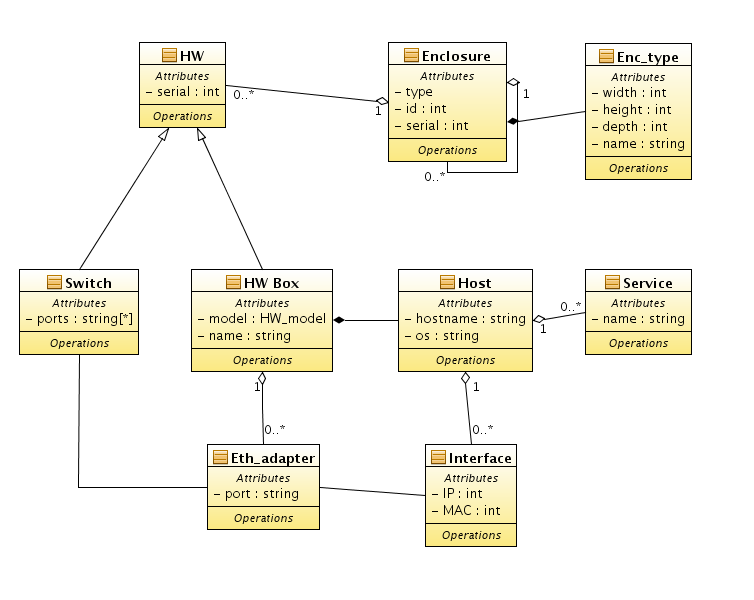
\includegraphics[width=14cm]{class_diagram.png}

This figure depicts the model of the data stored in the Database.  Each class
corresponds to a logical piece of infrastructure that we are modelling.

\subsection{Component Diagram}
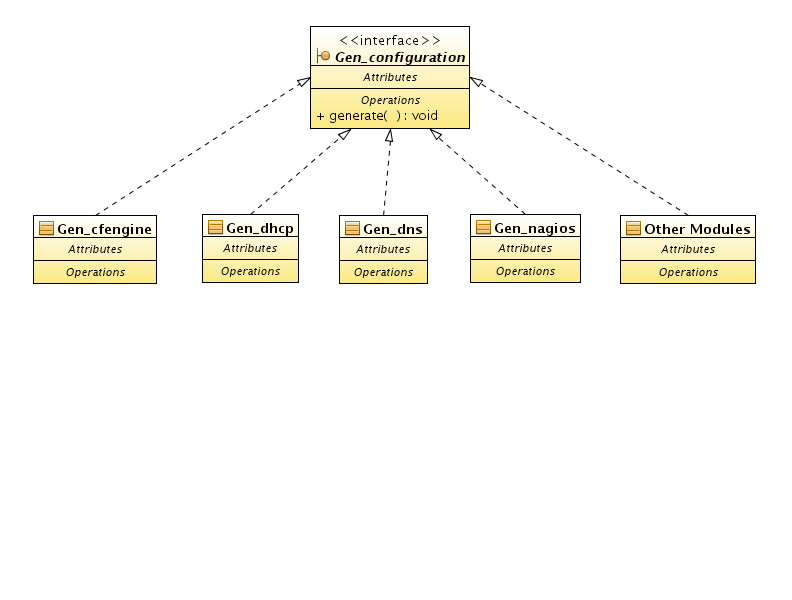
\includegraphics[width=14cm]{class_diagram_generators.png}

In this model we describe how are various components going to use the data from
the Database.  Please note that this is just a preliminary model which is
subject to change, especially due to some ongoing negotiations with the
Institute.

\section{Project Glossary}

For general overview and a glossary of terms used in this document, please have
a look at the ``Tool for Central Administration of a Grid Site'' document.

\end{document}
